\chapter{R Code and Generated Output}
\label{app:r-code}

This appendix illustrates how to present a reproducible statistical
calculation alongside its R code, numerical output, and figures. The examples
use the observations 1, 2, and 3 from Chapter~\ref{chap:normal-mean}. They
demonstrate presentation and computation rather than provide a substantive
data analysis.


The code and output below are generated with \texttt{knitr} from separate Rnw
files. Each file runs independently, and this appendix includes its generated
LaTeX with \verb|\input|. Edit the Rnw sources and rebuild to update both the
calculations and their displayed results; do not edit the generated tex files.


First, \texttt{Rnw/mean-ci.Rnw} computes the sample summaries and the
normal-model confidence interval derived in Chapter~\ref{chap:normal-mean}.
The calculation makes the connection between the formula and its numerical
implementation explicit.

% Generated with knitr; edit this Rnw source and rebuild, not the output tex.
\section{Normal-mean interval}
The following chunk calculates the summary statistics and confidence interval
for the illustrative observations in Chapter~\ref{chap:normal-mean}.
The units are arbitrary.

\begin{knitrout}
\definecolor{shadecolor}{rgb}{0.969, 0.969, 0.969}\color{fgcolor}\begin{kframe}
\begin{alltt}
\hldef{x} \hlkwb{<-} \hlkwd{c}\hldef{(}\hlnum{1}\hldef{,} \hlnum{2}\hldef{,} \hlnum{3}\hldef{)}
\hldef{n} \hlkwb{<-} \hlkwd{length}\hldef{(x)}
\hldef{x_bar} \hlkwb{<-} \hlkwd{mean}\hldef{(x)}
\hldef{s} \hlkwb{<-} \hlkwd{sd}\hldef{(x)}
\hldef{se} \hlkwb{<-} \hldef{s} \hlopt{/} \hlkwd{sqrt}\hldef{(n)}
\hldef{ci} \hlkwb{<-} \hldef{x_bar} \hlopt{+} \hlkwd{c}\hldef{(}\hlopt{-}\hlnum{1}\hldef{,} \hlnum{1}\hldef{)} \hlopt{*} \hlkwd{qt}\hldef{(}\hlnum{0.975}\hldef{,} \hlkwc{df} \hldef{= n} \hlopt{-} \hlnum{1}\hldef{)} \hlopt{*} \hldef{se}
\hlkwd{round}\hldef{(}\hlkwd{c}\hldef{(}\hlkwc{n} \hldef{= n,} \hlkwc{mean} \hldef{= x_bar,} \hlkwc{sd} \hldef{= s,} \hlkwc{se} \hldef{= se,}
        \hlkwc{lower} \hldef{= ci[}\hlnum{1}\hldef{],} \hlkwc{upper} \hldef{= ci[}\hlnum{2}\hldef{]),} \hlnum{3}\hldef{)}
\end{alltt}
\begin{verbatim}
##      n   mean     sd     se  lower  upper 
##  3.000  2.000  1.000  0.577 -0.484  4.484
\end{verbatim}
\end{kframe}
\end{knitrout}



Next, \texttt{Rnw/bootstrap.Rnw} implements the resampling procedure in
Algorithm~\ref{alg:bootstrap-mean}. The generated figure complements the
numerical output by showing the distribution of the bootstrap means.

% Generated with knitr; edit this Rnw source, not the output tex.


\section{Bootstrap calculation}
This chunk implements Algorithm~\ref{alg:bootstrap-mean}. The seed fixes the
random-number stream used for this demonstration. With only three
observations, the empirical distribution has very limited support; the
bootstrap interval below illustrates computation rather than reliable
coverage for a scientific application.

\begin{knitrout}
\definecolor{shadecolor}{rgb}{0.969, 0.969, 0.969}\color{fgcolor}\begin{kframe}
\begin{alltt}
\hlkwd{set.seed}\hldef{(}\hlnum{20260927}\hldef{)}
\hldef{B} \hlkwb{<-} \hlnum{2000L}
\hldef{alpha} \hlkwb{<-} \hlnum{0.05}
\hldef{boot_mean} \hlkwb{<-} \hlkwd{replicate}\hldef{(}
  \hldef{B,} \hlkwd{mean}\hldef{(}\hlkwd{sample}\hldef{(x,} \hlkwc{size} \hldef{= n,} \hlkwc{replace} \hldef{=} \hlnum{TRUE}\hldef{))}
\hldef{)}
\hlkwd{quantile}\hldef{(boot_mean,}
         \hlkwc{probs} \hldef{=} \hlkwd{c}\hldef{(alpha} \hlopt{/} \hlnum{2}\hldef{,} \hlnum{1} \hlopt{-} \hldef{alpha} \hlopt{/} \hlnum{2}\hldef{),} \hlkwc{names} \hldef{=} \hlnum{FALSE}\hldef{)}
\end{alltt}
\begin{verbatim}
## [1] 1 3
\end{verbatim}
\end{kframe}
\end{knitrout}

Report the seed, the number of resamples, the interval method, and software
versions in a reproducible
analysis. These bootstrap resamples are distinct from the independently
generated datasets used to estimate repeated-sampling coverage in a simulation
study.


\section{A figure generated by R}
Figure~\ref{fig:bootstrap-distribution} displays the empirical cumulative
distribution of the bootstrap means from Algorithm~\ref{alg:bootstrap-mean}.
Its steps reflect the limited support of the three-observation sample.
The vertical lines identify the observed mean and percentile endpoints.



\begin{knitrout}
\definecolor{shadecolor}{rgb}{0.969, 0.969, 0.969}\color{fgcolor}\begin{kframe}
\begin{alltt}
\hldef{endpoints} \hlkwb{<-} \hlkwd{quantile}\hldef{(}
  \hldef{boot_mean,} \hlkwc{probs} \hldef{=} \hlkwd{c}\hldef{(alpha} \hlopt{/} \hlnum{2}\hldef{,} \hlnum{1} \hlopt{-} \hldef{alpha} \hlopt{/} \hlnum{2}\hldef{),} \hlkwc{names} \hldef{=} \hlnum{FALSE}
\hldef{)}
\hlkwd{plot}\hldef{(}\hlkwd{ecdf}\hldef{(boot_mean),}
     \hlkwc{main} \hldef{=} \hlsng{""}\hldef{,} \hlkwc{xlab} \hldef{=} \hlsng{"Bootstrap sample mean"}\hldef{,}
     \hlkwc{ylab} \hldef{=} \hlsng{"Empirical cumulative probability"}\hldef{,}
     \hlkwc{verticals} \hldef{=} \hlnum{TRUE}\hldef{,} \hlkwc{do.points} \hldef{=} \hlnum{FALSE}\hldef{,} \hlkwc{xlim} \hldef{=} \hlkwd{c}\hldef{(}\hlnum{0.8}\hldef{,} \hlnum{3.2}\hldef{))}
\hlkwd{abline}\hldef{(}\hlkwc{v} \hldef{= x_bar,} \hlkwc{lty} \hldef{=} \hlnum{3}\hldef{)}
\hlkwd{abline}\hldef{(}\hlkwc{v} \hldef{= endpoints,} \hlkwc{lty} \hldef{=} \hlnum{2}\hldef{,} \hlkwc{col} \hldef{=} \hlsng{"blue"}\hldef{)}
\hlkwd{legend}\hldef{(}\hlsng{"topleft"}\hldef{,} \hlkwd{c}\hldef{(}\hlsng{"Observed mean"}\hldef{,} \hlsng{"Percentile endpoints"}\hldef{),}
       \hlkwc{lty} \hldef{=} \hlkwd{c}\hldef{(}\hlnum{3}\hldef{,} \hlnum{2}\hldef{),} \hlkwc{col} \hldef{=} \hlkwd{c}\hldef{(}\hlsng{"black"}\hldef{,} \hlsng{"blue"}\hldef{),} \hlkwc{bty} \hldef{=} \hlsng{"n"}\hldef{)}
\end{alltt}
\end{kframe}
\end{knitrout}

\begin{figure}[tbp]
\begin{knitrout}
\definecolor{shadecolor}{rgb}{0.969, 0.969, 0.969}\color{fgcolor}

{\centering 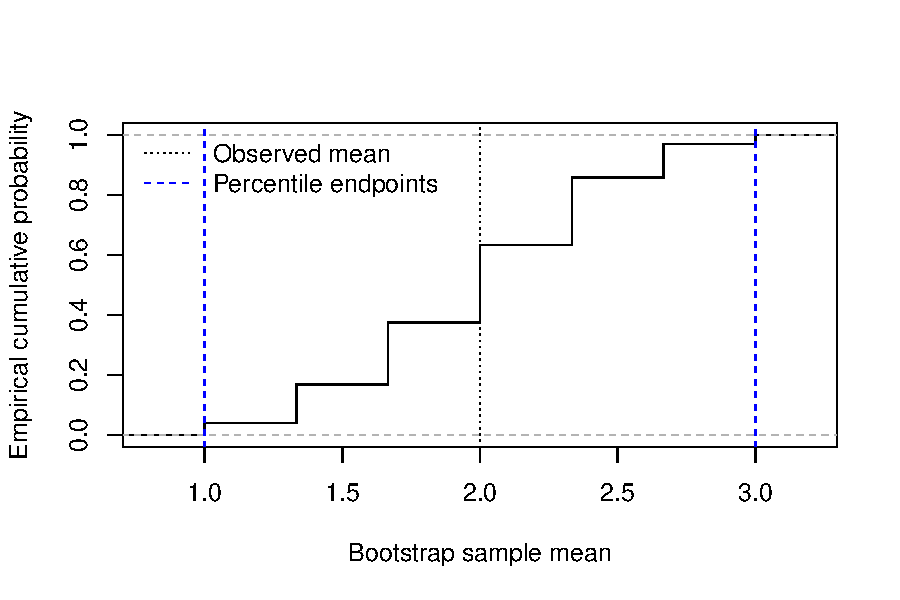
\includegraphics[width=\linewidth]{figures/bootstrap/bootstrap-distribution-1} 

}


\end{knitrout}

\caption[Empirical cumulative distribution of bootstrap means]{
Empirical cumulative distribution of 2,000 bootstrap means from the
observations 1, 2, and 3, using seed 20260927. The dotted line marks the
observed mean of 2; dashed lines mark the 95 percent percentile interval
endpoints of 1 and 3. This small-sample example illustrates computation,
not reliable coverage.}
\label{fig:bootstrap-distribution}
\end{figure}

Figure~\ref{fig:bootstrap-distribution} is generated by the R chunk.
Its caption and label are set explicitly with LaTeX commands in this Rnw
source. Use \verb|\ref| to refer to the figure number in the text.
The shorter caption appears in the list of figures; the full caption
explains the data and line styles.


\paragraph{Software versions.}
The following output records the versions used to generate this appendix.

\begin{knitrout}
\definecolor{shadecolor}{rgb}{0.969, 0.969, 0.969}\color{fgcolor}\begin{kframe}
\begin{verbatim}
## R version 4.6.1 (2026-06-24) 
## knitr 1.51
\end{verbatim}
\end{kframe}
\end{knitrout}



For a research application, accompany computational output with an
interpretation of what it establishes and which assumptions it requires.
Report relevant software versions and simulation settings, and use informative
captions and numbered cross-references to connect figures with the discussion.
Follow \citet{schifano2026statistical} for further guidance on statistical
writing and the presentation of tables and figures.
